\subsection{Experiment 2: Misuse of Model Selection Can Lead to Over-Optimistic Performance Estimates}

\begin{figure}[H]
    \centering
    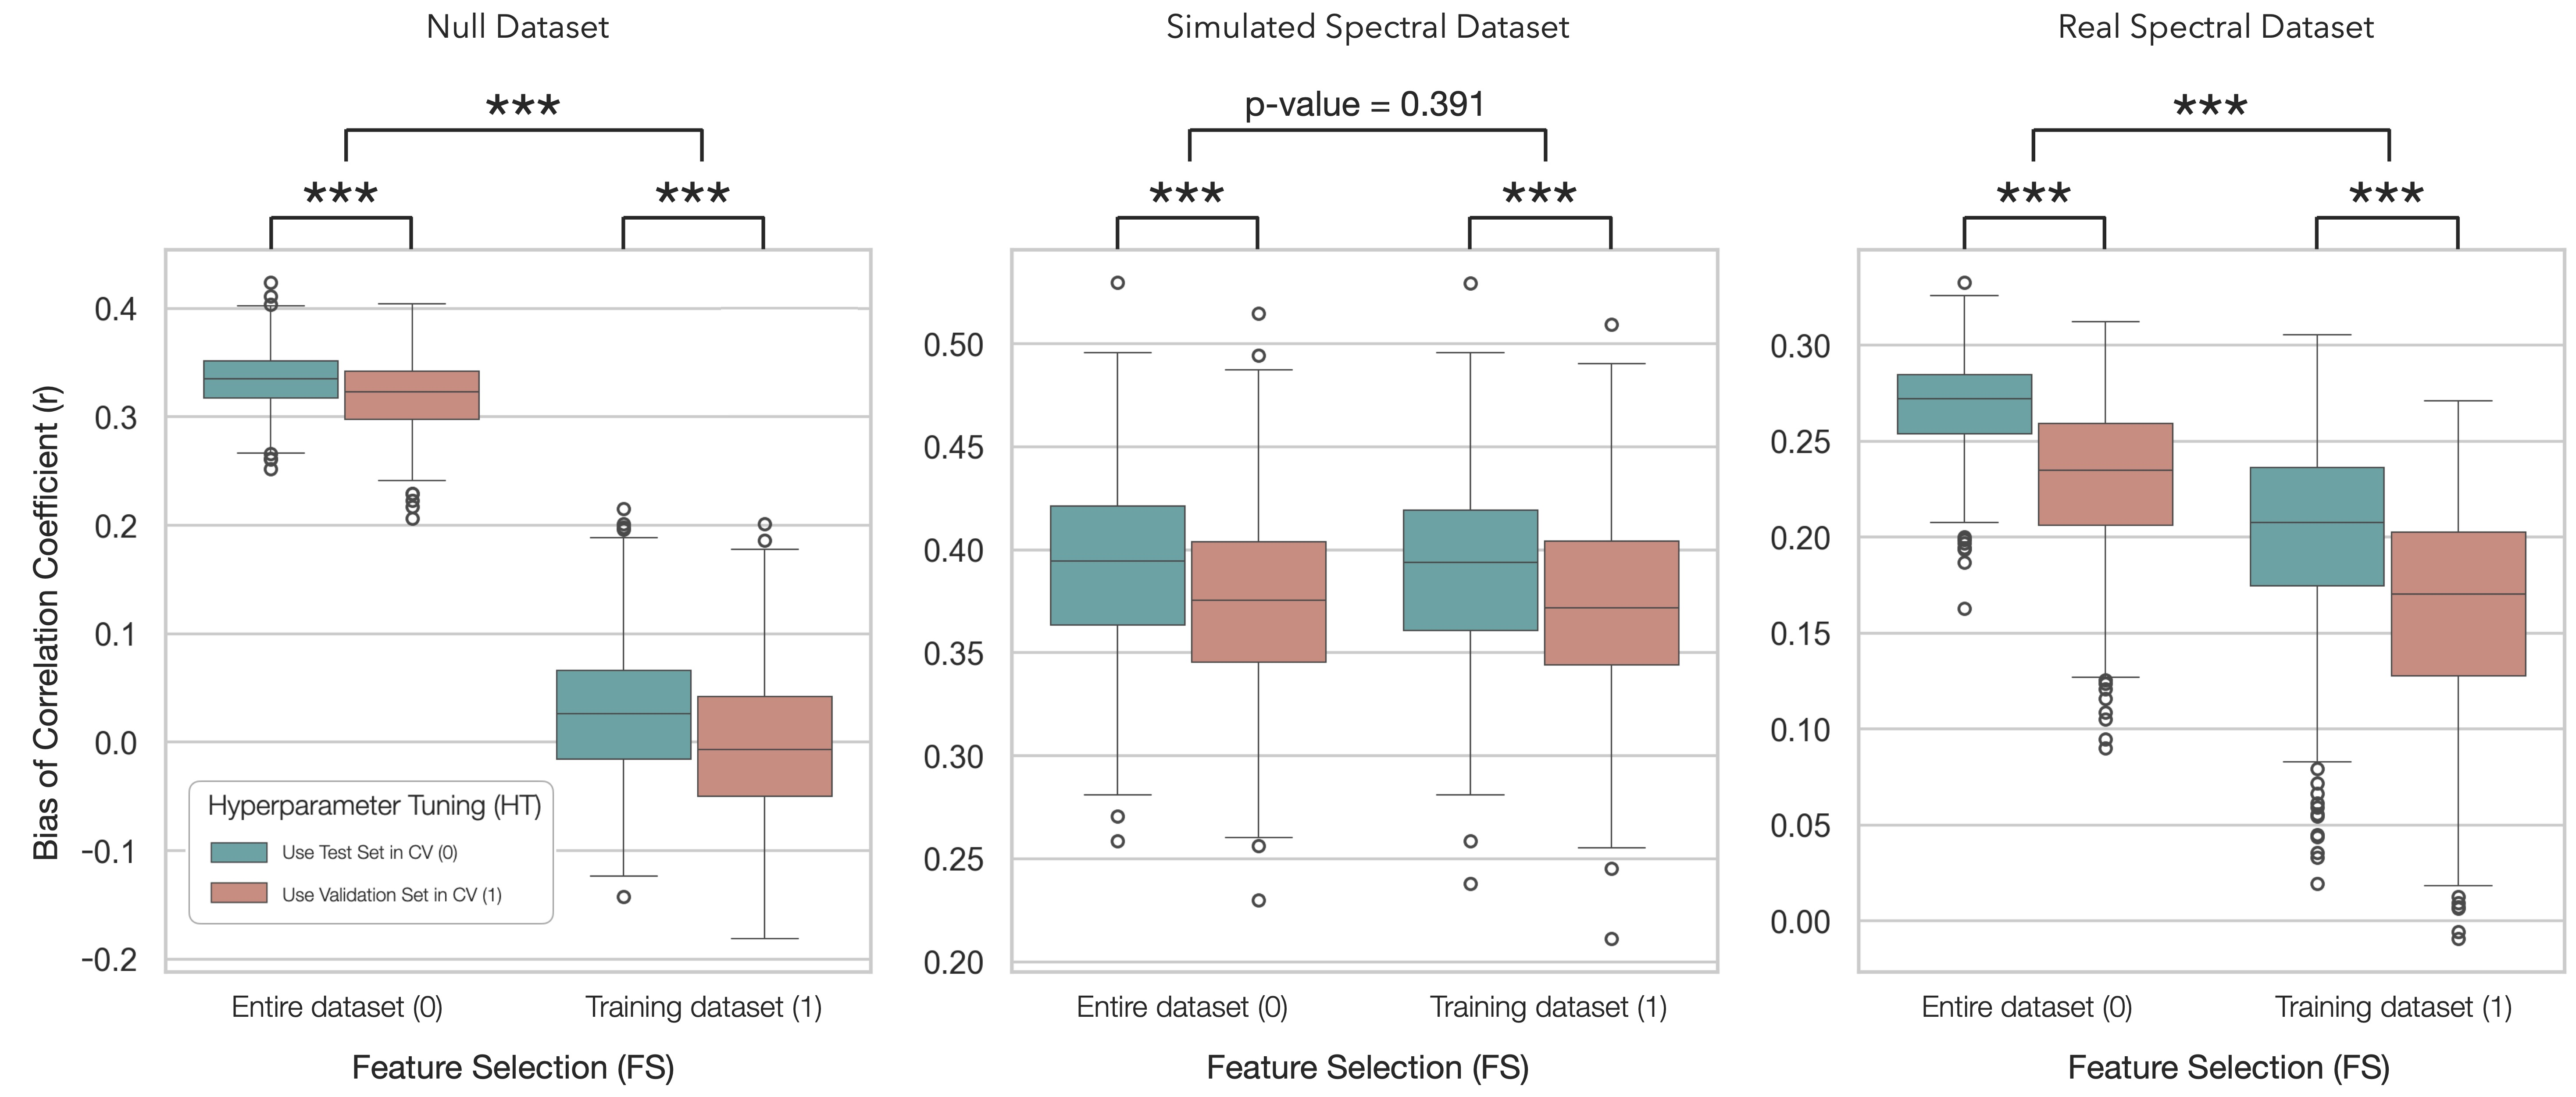
\includegraphics[width=1\textwidth]{fig_7.jpg}
    \caption{The evaluation bias of the four combinations of model selection strategies: “FS=0; HT=0”, “FS=0; HT=1”, “FS=1; HT=0”, “FS=1; HT=1” across three datasets. The significance level of the difference between the two strategies is noted as *** < 0.00001.}
    \label{fig:s2_results}
\end{figure}

With the exception of the feature selection procedure in the simulated spectral dataset, all other procedures that erroneously incorporate the testing set into the model selection process substantially inflate evaluation bias (Figure~\ref{fig:s2_results} and Table~\ref{tab:anova_r}). However, the magnitude of this inflation varies across datasets. In the null dataset, incorrectly performing feature selection leads to roughly a 30\% performance inflation; on the real dataset, a similar practice results in a 6\% inflation. By contrast, the simulated spectral dataset shows no measurable inflation, with only a negligible 0.02\% change in r. This minimal effect may stem from the degree to which the selected features contribute to predictive accuracy. If a model’s performance is comparable to that obtained through random feature selection, then leveraging the testing set for feature selection does not necessarily boost performance. Such a scenario is more plausible in datasets with high multicollinearity, where multiple features correlate strongly, making any subset of features effectively representative of the entire feature space.

On the other hand, using the entire dataset to perform hyperparameter tuning substantially inflates performance in all three datasets—by approximately 2.5\% in the null dataset, 1.5\% in the simulated spectral dataset, and nearly 4\% in the real spectral dataset. It is worth noting that these estimates arise from a relatively small search space of only six hyperparameter combinations. In contemporary machine learning, hyperparameter spaces can be far larger, especially for deep learning models in which the architectures themselves are highly configurable, involving potentially millions of parameters. Even minor alterations (e.g., changing the kernel size in a convolutional layer) may markedly affect model performance in such complex settings \citep{zoph_neural_2017}.

Model selection practices are critical in many precision agricultural applications. It is important to note that feature selection is not entirely prohibited from using the entire dataset, especially when employing unsupervised feature selection methods, such as the successive projections algorithm (SPA) \citep{soares_successive_2013}. These methods consider feature redundancy and select the most informative features without incorporating information from the target variable in the testing set. For example, Zhang et al. (2019) leveraged ground-based hyperspectral sensors to detect weed species in rice fields \citep{zhang_automated_2019}. Even after preprocessing and discarding spectral bands with high fluctuations due to hardware limitations, 470 bands remained for consideration. The SPA method was employed to select the most informative bands for the prediction task, ultimately identifying six key bands that also match the past literature on weed detection. This procedure is considered unbiased, as the feature selection was not explicitly performed to maximize model performance.

The same study demonstrated good practices in hyperparameter tuning. Within each training fold, a nested 5-fold cross-validation was implemented to identify the optimal hyperparameter combinations. For the random forest model, the number of trees and the spectral bands considered for splits were tuned during classifier development. Similarly, for the SVM model, the best regularization parameter $C$ and kernel function were identified to avoid overfitting. Other studies have adopted similar practices. For instance, Shahinfar et al. (2019) used a large dataset of sheep growth management records to predict carcass traits, including birth weight, age at slaughter, and breeding values for fat composition from ancestors \citep{shahinfar_prediction_2019}. Given the large feature space, careful hyperparameter tuning was essential to prevent overfitting. Shahinfar et al. employed nested cross-validation to select the optimal number of decision trees and bootstrap samples for the random forest model. These examples illustrate the importance of rigorous feature selection and hyperparameter tuning to enhance model reliability and generalizability in precision agricultural studies.

Collectively, these findings underscore the importance of rigorous CV practices in model selection, particularly for feature selection and hyperparameter tuning, to achieve accurate performance estimates and robust generalizability in predictive modeling.
